\documentclass[12pt,a4paper]{report}
\setlength\textwidth{145mm}
\setlength\textheight{247mm}
\setlength\oddsidemargin{15mm}
\setlength\evensidemargin{15mm}
\setlength\topmargin{0mm}
\setlength\headsep{0mm}
\setlength\headheight{0mm}
% \openright makes the following text appear on a right-hand page
\let\openright=\clearpage

%% Settings for two-sided (duplex) printing
% \documentclass[12pt,a4paper,twoside,openright]{report}
% \setlength\textwidth{145mm}
% \setlength\textheight{247mm}
% \setlength\oddsidemargin{14.2mm}
% \setlength\evensidemargin{0mm}
% \setlength\topmargin{0mm}
% \setlength\headsep{0mm}
% \setlength\headheight{0mm}
% \let\openright=\cleardoublepage

%% Character encoding: usually latin2, cp1250 or utf8:
\usepackage[utf8]{inputenc}


%% Further useful packages (included in most LaTeX distributions)
\usepackage{amsmath}        % extensions for typesetting of math
\usepackage{amsfonts}       % math fonts
\usepackage{amsthm}         % theorems, definitions, etc.
\usepackage{bm}             % boldface symbols (\bm)
\usepackage{graphicx}       % embedding of pictures
\usepackage{fancyvrb}       % improved verbatim environment
\usepackage{dcolumn}        % improved alignment of table columns
\usepackage{booktabs}       % improved horizontal lines in tables
\usepackage{paralist}       % improved enumerate and itemize
\usepackage[pdftex,dvipsnames]{xcolor}  % typesetting in color

\usepackage{cite}
\usepackage[colorinlistoftodos,prependcaption,textsize=tiny]{todonotes}
\usepackage{xargs}


\newcommandx{\problem}[2][1=]{\todo[linecolor=red,backgroundcolor=red!25,bordercolor=red,#1]{#2}}
\newcommandx{\todoo}[2][1=]{\todo[linecolor=blue,backgroundcolor=blue!25,bordercolor=blue,#1]{#2}}
\newcommandx{\note}[2][1=]{\todo[linecolor=OliveGreen,backgroundcolor=OliveGreen!25,bordercolor=OliveGreen,#1]{#2}}
\newcommandx{\unsure}[2][1=]{\todo[linecolor=Plum,backgroundcolor=Plum!25,bordercolor=Plum,#1]{#2}}



\begin{document}
\chapter{Numerical study}
To reiterate, the model has five different parameters. The hardcore parameters are $\epsilon$ and $ \alpha$ controlling the minimum face area and maximum circumradius, respectivelly. The smooth interaction parameter $\theta$ controls the surface area of the cells. Finally the intensity $z$ of the underlying Poisson process and $W$, the maximum possible weight for a point. Throughout this chapter, some parameters will remain constant, namely $z = 500$ and $W = 0.01$.

For the purposes of estimation, the hardcore parameter $\epsilon$ is not introduced, as it has not been theoretically proven that non-scalar hardcore parameter would lead to consistent estimation even in the two-dimensional Delaunay case (although [DereudreLavancier07] believes it is the case). \newline


\note[inline]{The parameter $\alpha$ does not seem to pose any problems for the simulation}
\todoo[inline]{Include some simulations with $\alpha$}
 
\section{Simulation}

\begin{figure}[h]
    \centering
    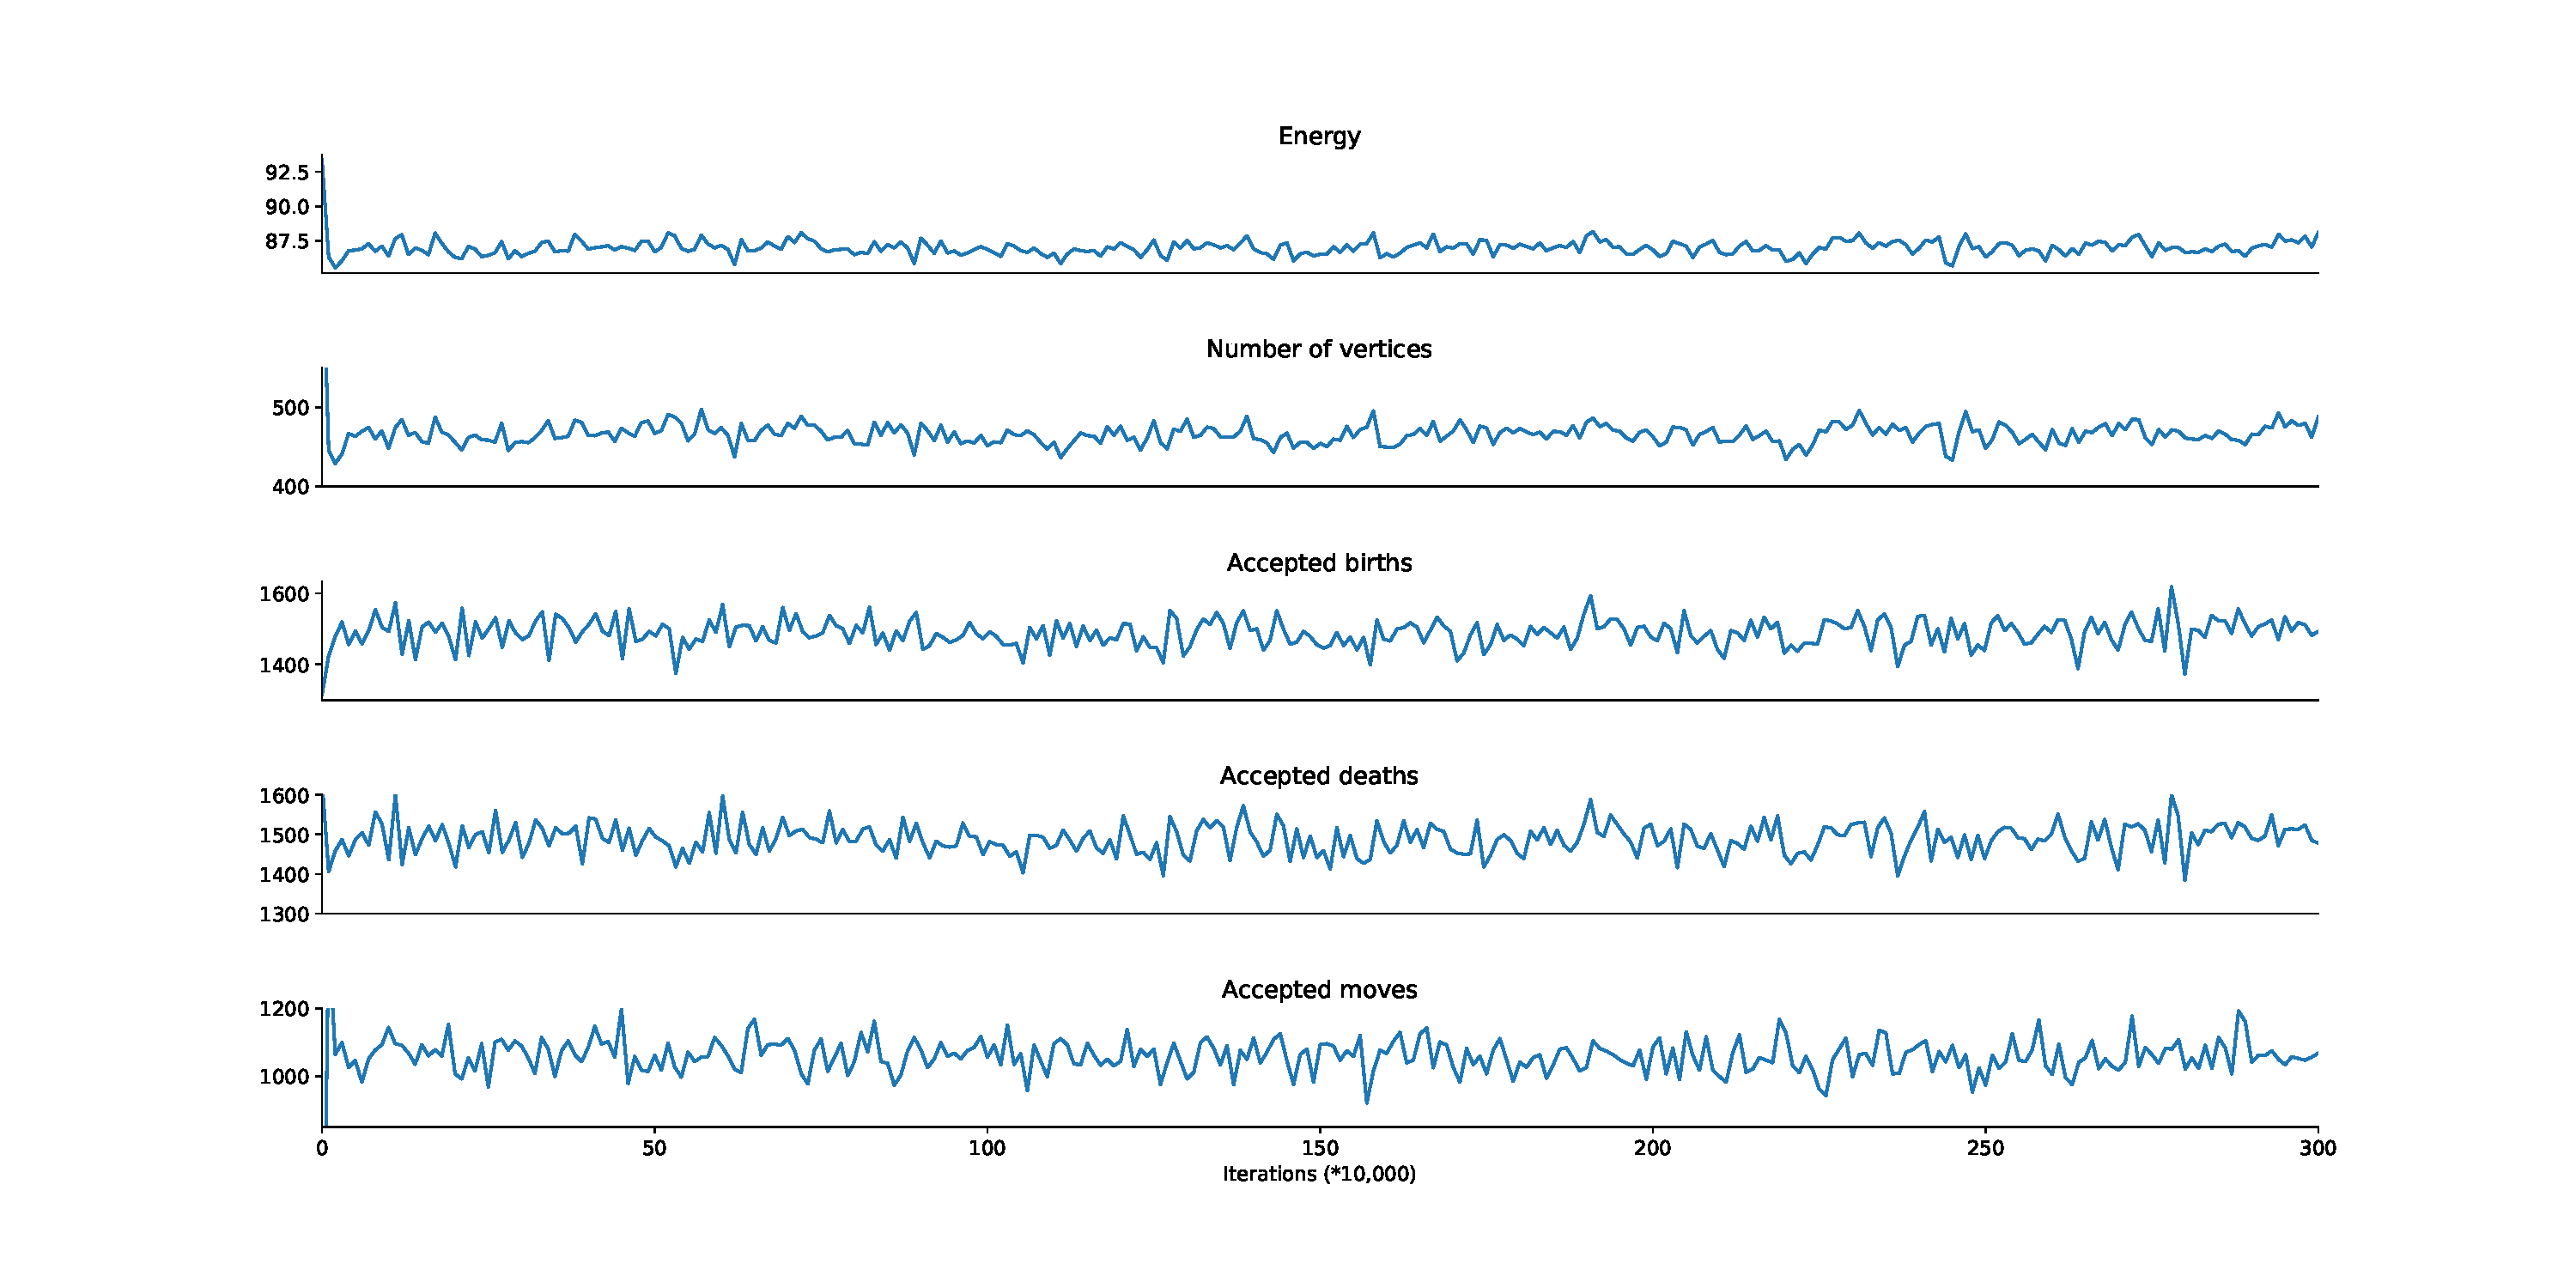
\includegraphics[width=1\textwidth]{images/convergence.pdf}
    \caption{Convergence metrics. Total number of iterations: $3\times 10^6$. $\theta=2, \alpha = 0.15, z = 500, W = 0.01$}
    \label{fig:conv}
\end{figure}

As mentioned in a previous section, the simulation is done through a Birth-Death-Move algorithm. As such it is only approximative in nature and thus appropriate visual aids have to be used in order to monitor the convergence. Figure \ref{fig:conv}  shows the visual aids for one tessellation. These suggest that the Markov chain has entered a high-probability region of the distribution and stayed in it. 


\subsection{The role of $\theta$}
\begin{figure}[h]
    \centering
    \includegraphics[width=1\textwidth]{images/facets.pdf}
    \caption{Facet volumes for $\alpha = 0.15, z = 500, W = 0.01$ with $\theta=0.1$ and $\theta=10$}
    \label{fig:facets}
\end{figure}


\begin{figure}[h]
    \centering
    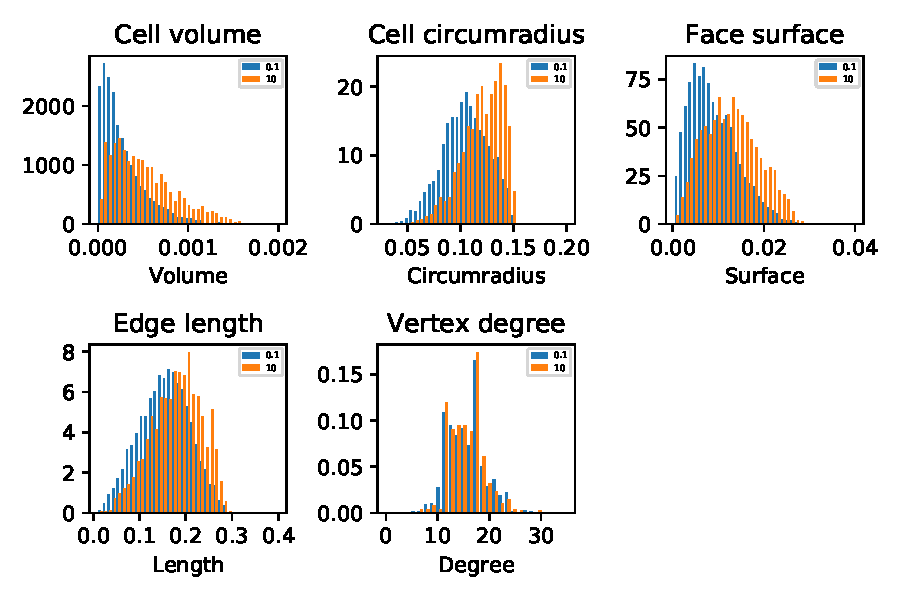
\includegraphics[width=1\textwidth]{images/facets_extr.pdf}
    \caption{Facet volumes for $\alpha = 0.15, z = 500, W = 0.01$ with $\theta=0.1$ and $\theta=100$}
    \label{fig:facets_extr}
\end{figure}
The parameter $\theta$ multiplies the surface area of the cells in the sum. A higher $\theta$ means that surface area will have a greater effect on the energy. In practice, this forces the cells to be as large as possible (within limits of the hardcore interaction) in order to minimize the total surface area. A lower $\theta$ then in turn results in a greater number of smaller cells. This is exemplified in figures \ref{fig:facets} and \ref{fig:facets_extr} where $\theta=0.1$ is contrasted with $\theta=10$ and $\theta=100$ and the facet volume distributions are shifted to the right. This is most pronounced in case of circumradii, where the distribution in case of $\theta=100$ amasses at the boundary of $0.15$. 

\problem[inline]{Multi-modality in edge length and vertex degree is quite suspicious - boundary problems?}
\problem[inline]{The y-axes don't make much sense, force matplotlib to show probabilities, rather than densities}

\subsection{$\theta < 0$}
In the case when $\theta$ is negative, the energy-surface relationship is inverted and the algorithm will attempt to maximize the surface area by converging into configurations with a large number of small cells. A comparison is provided in figure \ref{fig:facets_neg}. \newline 

\unsure[inline]{Is this a big enough difference? Can we conclude the simulation works?}
\todoo[inline]{Explore further, provide plots,reasons,..}

\section{Estimation}
\begin{figure}[h]
    \centering
    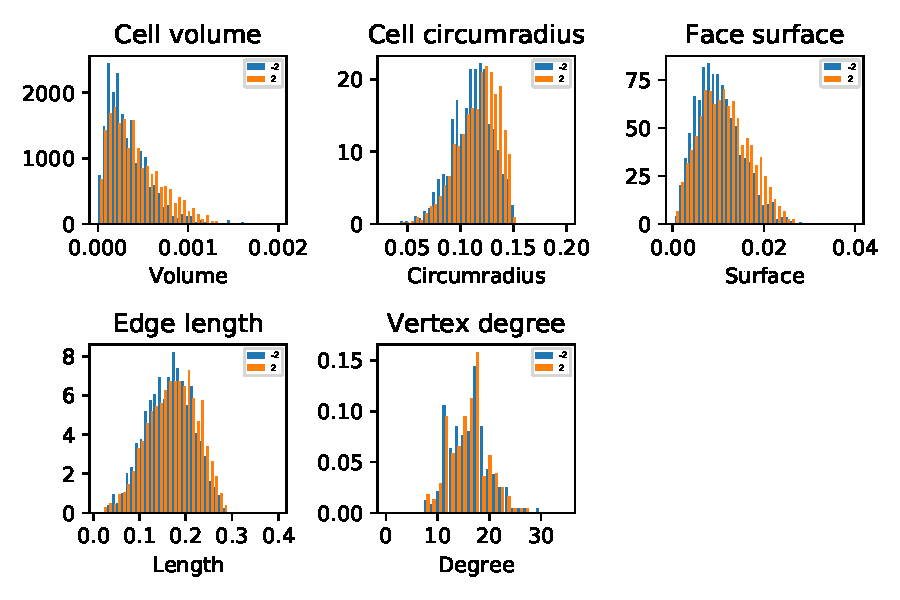
\includegraphics[width=1\textwidth]{images/facets_neg.pdf}
    \caption{Facet volumes for $\alpha = 0.15, z = 500, W = 0.01$ with $\theta=-2$ and $\theta=2$}
    \label{fig:facets_neg}
\end{figure}


\begin{figure}[h]
    \centering
    \includegraphics[width=1\textwidth]{images/estimates.pdf}
    \caption{Estimates for a model with $\theta=2, \alpha = 0.2, z = 500, W = 0.01$ with $303$ simulations}
    \label{fig:estimates}
\end{figure}

\begin{figure}[h]
    \centering
    \includegraphics[width=1\textwidth]{images/estimates_neg.pdf}
    \caption{Estimates for a model with $\theta=-2, \alpha = 0.15, z = 500, W = 0.01$ with only about $8$ simulations.}
    \label{fig:estimates_neg}
\end{figure}
The estimation results for $\theta=2$ for $303$ realizations are shown in figure \ref{fig:estimates}. The graph shows qualitatively correct results, sadly, the values are overestimated with no clear reason why. A small number of realizations ($8$) was done for $\theta=-2$ as can be seen in figure \ref{fig:estimates_neg}, which suggests an even worse results. It must also be mentioned that both cases, particularly the negative $\theta$ case sometimes produced nonsensical $\hat\theta$ values of $10000$. \newline

\todoo[inline]{Compare estimation with and without $\alpha$ present.}
\problem[inline]{Estimation seems to sometimes result in nonsensical values, especially with $\theta<0$, investigate why}







%%%%%%%%%%%%%%%%%%%%%%%%%%%%%%%%%%%%%%%%

\bibliography{bibliography}
\bibliographystyle{plain}


\listoftodos



\end{document}
